\chapter*{Overall description}
\addcontentsline{toc}{chapter}{Overall description}

\section*{Product features}
\addcontentsline{toc}{section}{Product features}

All developed hardware presented as logisim circuits.

Product implements cellular automaton with 32x32 game field and set of rules, including:

\begin{itemize}
	\item \textbf{Born} - set of integers from 0 to 8, specifying, with what amount of alive neighbours cell will become alive.
	\item \textbf{Surv} - set of integers from 0 to 8, specifying, with what amount of alive neighbours cell will survive.
	\item \textbf{Speed} - integer from 0 to 3, specifying game speed.
\end{itemize}

CdM-16 processor with single banked RAM chip forms heart of product, it processes user input, manages templates (some specified part of game field, stored in one of 5 slots) and handles errors.

CdM-16 processor has the ability to communicate with cellular automaton, within this communication processor can read and modify automaton state.

Product allows user to connect to it with external terminal through UART. UART will use interrupts to trigger printing of hello message and processing of data, sended by user. With this connection user can do following:

\begin{itemize}
	\item Modify game field
	\item Modify rules
	\item Control game flow, start or pause game, trigger single iteration of game
	\item Save and paste templates
\end{itemize}

\begin{figure}[ht]
	\centering
	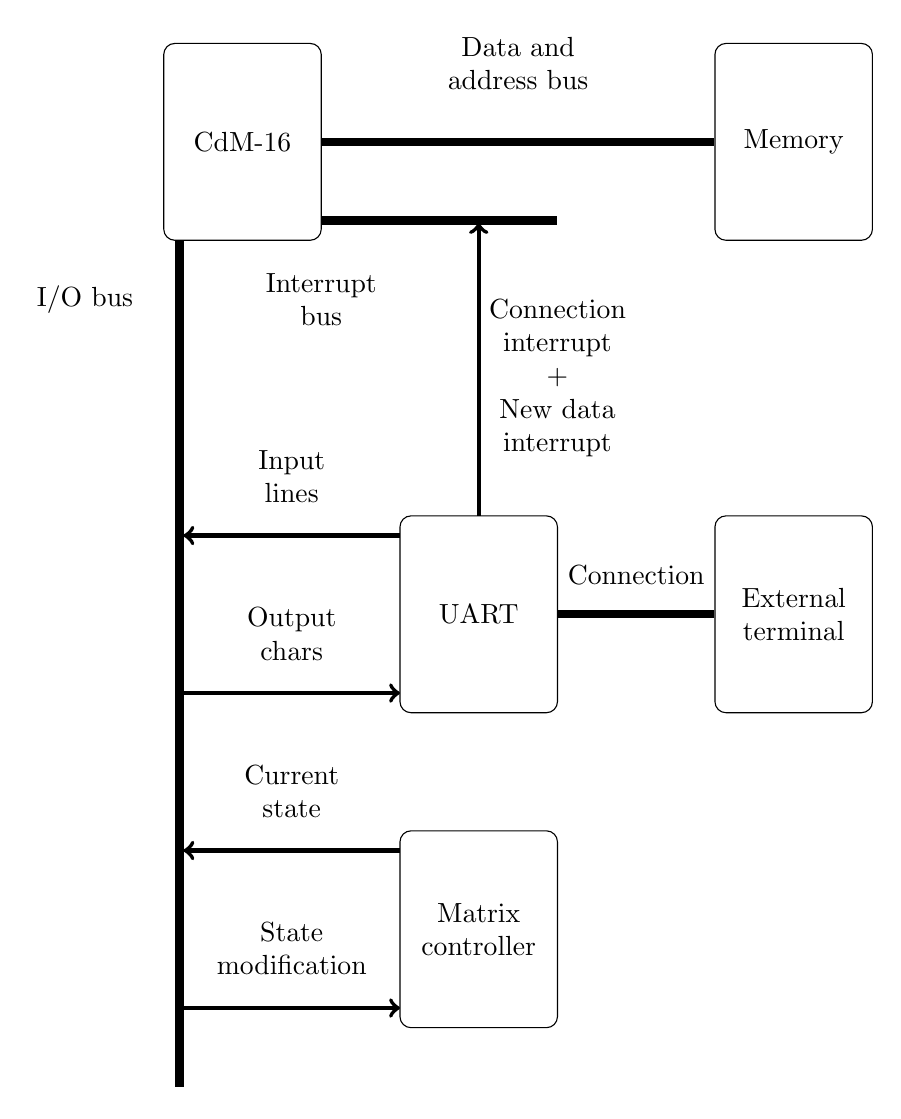
\begin{tikzpicture}[main/.style={draw, rounded corners, minimum width = 20mm, minimum height = 25mm}]
		\node[main] (cdm) {CdM-16};	
		\node[main] at (7,0) (mem) {Memory};
		\node[main, align=center] at (3,-10) (mcontr) {Matrix\\controller};
		\node[main] at (3,-6) (ucontr) {UART};
		\node[main, align=center] at (7,-6) (extt) {External\\terminal};

		\node[align=center] at (3.5, 1) {Data and\\address bus};
		\draw[line width = 3pt] (cdm) -- (mem);

		\node[align=center] at (1, -2) {Interrupt\\bus};
		\draw[line width = 3pt] (1, -1) -- (4, -1);

		\node at (-2, -2) {I/O bus};
		\draw[line width = 3pt] (-0.8, -1.25) -- (-0.8, -12);

		\node[align=center] at (0.625, -4.25) {Input\\lines};
		\path[->, line width = 1.5pt] (2,-5) edge (-0.75, -5);
		\node[align=center] at (0.625, -6.25) {Output\\chars};
		\path[->, line width = 1.5pt] (-0.75, -7) edge (2,-7);

		\node[align=center] at (0.625, -8.25) {Current\\state};
		\path[->, line width = 1.5pt] (2,-9) edge (-0.75, -9);
		\node[align=center] at (0.625, -10.25) {State\\modification};
		\path[->, line width = 1.5pt] (-0.75, -11) edge (2,-11);

		\node[align=center] at (4, -3) {Connection\\interrupt\\+\\New data\\interrupt};
		\path[->, line width = 1.5pt] (3,-4.75) edge (3, -1.03125);

		\node at (5, -5.5) {Connection};
		\draw[line width = 3pt] (extt) -- (ucontr);
	\end{tikzpicture}
	\caption{General design}
\end{figure}

\section*{Operating environment}
\addcontentsline{toc}{section}{Operating environment}

For running product you need:

\begin{itemize}
	\item Logisim
	\item \href{https://github.com/cdm-processors/cdm-devkit}{CdM-devkit} ver. 0.2.2 or above JAR libraries (cdm16 emulator, banked memory)
	\item UART JAR library
	\item External terminal with ability to connect to UART via telnet protocol.
\end{itemize}

For building purposes you need:

\begin{itemize}
	\item \href{https://github.com/Proletcultist/cdm-devkit-macro-improvements}{This} fork of CdM-devkit
	\item Some make implementation (such as GNU make)
\end{itemize}
